\documentclass[aspectratio=169,12pt,t]{beamer}

\usepackage{amsmath,amssymb}
\usepackage{tikz}
\setbeamercolor{normal text}{fg=black,bg=white}
\setbeamercolor{structure}{fg=black}
\setbeamercolor{frametitle}{fg=black,bg=white}
\setbeamerfont{frametitle}{size=\Large,series=\bfseries}
\setbeamersize{text margin left=1cm,text margin right=1cm}
\setbeamertemplate{navigation symbols}{}
\setbeamertemplate{itemize item}{\textbullet}
\definecolor{cyclecolor}{HTML}{8C2858}
\newcommand{\definedterm}[1]{\textcolor{cyclecolor}{\textbf{#1}}}

\begin{document}

\begin{frame}[plain,c]
  \centering
  {\LARGE\bfseries Proof Simplification\\for Barnette's Conjecture\par}
  \vspace{1em}
  Anouk Brose (UC Davis)\par
  Tom de Groot (independent)\par
  Santiago Morales Duarte (UC Davis)\par
  \vspace{0.75em}
  {\small\color{black!60}Mathathon, November 13--15, 2026\par}
  \begin{tikzpicture}[remember picture,overlay,inner sep=0pt]
    \node[anchor=west,xshift=1cm,yshift=9mm] at (current page.south west)
      {
\includegraphics[width=2cm]{slide-assets/sair-logo.jpg}};
    \node[yshift=9mm] at (current page.south)
      {
\includegraphics[width=2cm]{slide-assets/caltech-logo.jpg}};
    \node[anchor=east,xshift=-1cm,yshift=9mm] at (current page.south east)
      {
\includegraphics[viewport=33bp 62.5bp 110bp 115bp,clip,height=0.9cm]{slide-assets/mathathon-reference.png}};
  \end{tikzpicture}
\end{frame}

\begin{frame}[c]{Icosian Game}
  \centering
  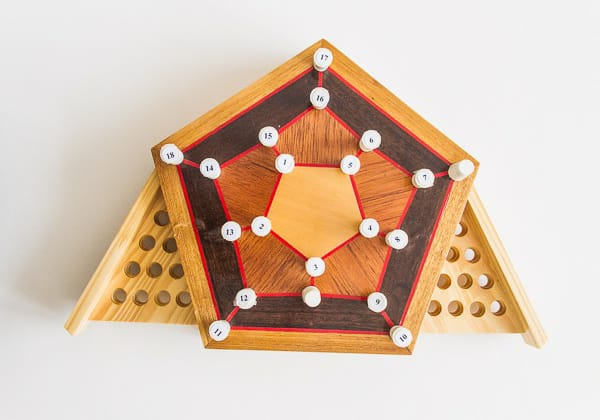
\includegraphics[width=0.8\linewidth,height=5.1cm,keepaspectratio]{slide-assets/icosian-game.jpg}\par
  \smallskip
  {\small Hamilton's Icosian game (1857)\par}
  {\scriptsize A cycle through every vertex of a dodecahedron\par}
  {\tiny\color{black!65}\href{https://commons.wikimedia.org/wiki/File:Jogo_icosiano_01.jpg}{Matemateca (IME/USP)/Alisson Ricardo}, \href{https://creativecommons.org/licenses/by-sa/4.0/}{CC BY-SA 4.0}\par}
\end{frame}

\begin{frame}{Barnette's Conjecture (1969)}
  \noindent\resizebox{\linewidth}{!}{%
    \bfseries\boldmath
    \begin{tabular}{@{}l@{}}
      Every \alt<2->{\definedterm{simple \(3\)-polytope}}{simple \(3\)-polytope} with even-sided faces has a
      \alt<3->{\definedterm{Hamiltonian}}{Hamiltonian} vertex-edge graph.\\[0.55em]
      \uncover<2->{\footnotesize\mdseries\unboldmath\itshape\color{cyclecolor}
        A \(3\)-polytope is the convex hull of finitely many points that affinely span \(\mathbb{R}^3\).}\\
      \uncover<2->{\footnotesize\mdseries\itshape\color{cyclecolor}
        It is simple if every vertex has degree three.}\\[0.2em]
      \uncover<3->{\footnotesize\mdseries\itshape\color{cyclecolor}
        A Hamiltonian cycle in a graph is a cycle that visits each vertex exactly once.}\\[1.15em]
      \uncover<4->{\(\Longleftrightarrow\)\enspace Every \(3\)-connected, cubic, bipartite planar graph has a
        \definedterm{Hamiltonian cycle}.{\mdseries~\cite{barnette-conjecture,barnette-equivalence}}}
    \end{tabular}%
  }\par
  \vspace{1.5em}

  \begin{columns}[c,onlytextwidth]
    \begin{column}{0.48\textwidth}
      \centering
      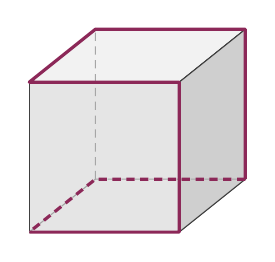
\begin{tikzpicture}[scale=1.12,line join=round,draw=black!75]
        \filldraw[fill=black!5] (0,1.7) -- (1.7,1.7) -- (2.45,2.3) -- (0.75,2.3) -- cycle;
        \filldraw[fill=black!19] (1.7,0) -- (2.45,0.6) -- (2.45,2.3) -- (1.7,1.7) -- cycle;
        \filldraw[fill=black!10] (0,0) rectangle (1.7,1.7);
        \draw[densely dashed,black!35]
          (0,0) -- (0.75,0.6) -- (2.45,0.6)
          (0.75,0.6) -- (0.75,2.3);
        \only<3->{%
          \draw[cyclecolor,line width=1.15pt]
            (0,0) -- (1.7,0) -- (1.7,1.7) -- (0,1.7)
            -- (0.75,2.3) -- (2.45,2.3) -- (2.45,0.6);
          \draw[cyclecolor,line width=1.15pt,densely dashed]
            (2.45,0.6) -- (0.75,0.6) -- (0,0);
        }
      \end{tikzpicture}\par
      {\scriptsize The \(3\)-cube\par}
    \end{column}
    \begin{column}{0.48\textwidth}
      \centering
      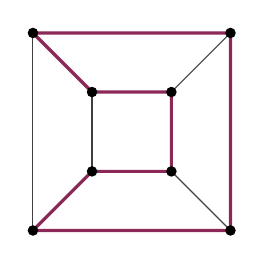
\begin{tikzpicture}[scale=1.12,draw=black!75]
        \draw (-1.12,-1.12) rectangle (1.12,1.12);
        \draw (-0.45,-0.45) rectangle (0.45,0.45);
        \foreach \x in {-1,1} {
          \foreach \y in {-1,1} {
            \draw ({0.45*\x},{0.45*\y}) -- ({1.12*\x},{1.12*\y});
          }
        }
        \only<3->{%
          \draw[cyclecolor,line width=1.15pt,line join=round]
            (-1.12,-1.12) -- (1.12,-1.12) -- (1.12,1.12) -- (-1.12,1.12)
            -- (-0.45,0.45) -- (0.45,0.45) -- (0.45,-0.45) -- (-0.45,-0.45)
            -- cycle;
        }
        \foreach \x in {-1,1}
          \foreach \y in {-1,1}
            \foreach \r in {0.45,1.12}
              \fill ({\r*\x},{\r*\y}) circle (1.7pt);
      \end{tikzpicture}\par
      {\scriptsize Vertex-edge graph of the \(3\)-cube\par}
    \end{column}
  \end{columns}
\end{frame}

\begin{frame}[c]{Motivation and Background}
  \begin{columns}[c,onlytextwidth]
    \begin{column}{0.70\textwidth}
      \small
      \setlength{\leftmargini}{1em}
      \begin{itemize}[<+->]
        \setlength{\itemsep}{0.65em}
        \item Tait (1884) wanted to prove the four-color theorem via Hamiltonian cycles in simple \(3\)-polytopes.
        \item Tutte (1946) found a non-Hamiltonian simple \(3\)-polytope.
        \item Barnette (1969) added the bipartite assumption.
        \item Goodey (1975) proved the case with only quadrilateral and hexagonal faces.
        \item Gorsky et al. (2023) proved equivalence to a strengthening of the conjecture with Pfaffian graphs.
      \end{itemize}
    \end{column}
    \begin{column}{0.26\textwidth}
      \centering
      \uncover<2->{%
        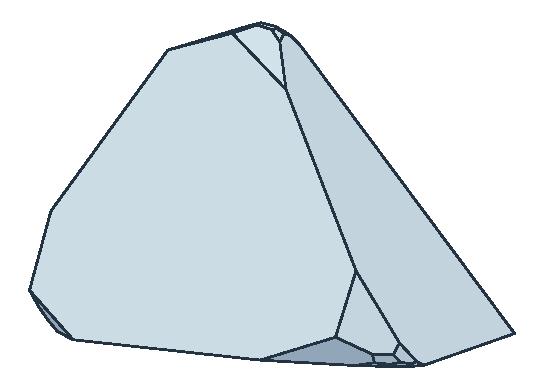
\includegraphics[width=\linewidth,height=2.15cm,keepaspectratio]{slide-assets/tutte-polytope.pdf}\par
        \vspace{0.65em}
        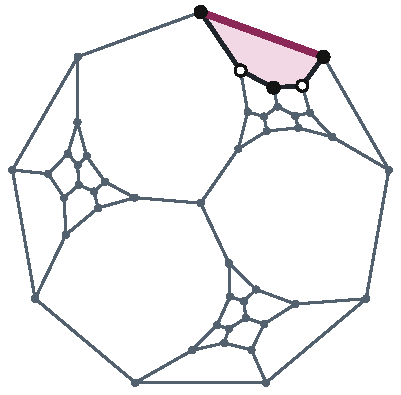
\includegraphics[width=\linewidth,height=2.15cm,keepaspectratio]{slide-assets/tutte-graph-original.pdf}\par
        \smallskip
        {\scriptsize Tutte's non-Hamiltonian polytope\par}
      }
    \end{column}
  \end{columns}
  \par\vspace{1.45em}
  \uncover<6->{\textbf{OpenAI released a proof of Barnette's conjecture on October 6, 2026.}~\cite{barnette-proof,openai-release}\par}
\end{frame}

\begin{frame}[c]{Our Contributions}
  \setbeamertemplate{enumerate item}{\large\bfseries\insertenumlabel.}
  \setbeamercolor{enumerate item}{fg=black}
  \setlength{\leftmargini}{0.7em}
  \small
  \begin{enumerate}[<+->]
    \setlength{\itemsep}{1.15em}
    \item {\large\bfseries Human expertise in geometric combinatorics}\par
      \vspace{0.15em}
      We verified most of the proof and are refactoring it: simplifying, adding necessary citations, differentiating key steps from smaller details.\par
      {\footnotesize\itshape\color{black!65}
        OpenAI released the paper as a preprint without peer review.\par}
    \item {\large\bfseries Interactive website}\par
      \vspace{0.15em}
      We are building a website and game to guide readers through the proof step by step.
    \item {\large\bfseries Proof simplification}\par
      \vspace{0.15em}
      We reduced the construction of a Hamiltonian cycle from six steps to four.
    \item {\large\bfseries Implemented algorithm to find a Hamiltonian cycle}
  \end{enumerate}
\end{frame}

\begin{frame}[c]{What do AI proofs lack, and what can humans add?}
  \setlength{\leftmargini}{1em}
  \begin{itemize}[<+->]
    \setlength{\itemsep}{0.9em}
    \item \textbf{Human intuition:} Choose representative examples that clarify the proof.
    \item \textbf{Proof structure:} Distinguish the key steps from smaller details.
    \item \textbf{Reasoned choices:} Revisit decisions the AI proof leaves unexplained and make informed decisions.
    \item \textbf{Credit and novelty:} Credit key ideas from earlier work and explain which steps are new.
    \item \textbf{Notation and naming:} Use standard notation and naming conventions.
  \end{itemize}
  \vspace{0.65em}
  \uncover<6->{\noindent
    \makebox[\linewidth][c]{\fontsize{11.5}{14}\selectfont\textcolor{cyclecolor}{Use AI for quality over quantity to produce \textbf{better} papers, expositions, and applications.}}\par}
\end{frame}

\begin{frame}[plain,c]
  \centering
  {\LARGE\bfseries Proof Walkthrough\par}
  \vspace{0.75em}
  {\small\href{https://tomodovodoo.github.io/mathathon-Barnette-s-Conjecture/barnette-proof-walkthrough.html}{\textcolor{cyclecolor}{\underline{Open the interactive walkthrough}}}\par}
\end{frame}

\begin{frame}[c]{Future Goals}
  \setlength{\leftmargini}{1em}
  \begin{itemize}
    \setlength{\itemsep}{0.7em}
    \item {\bfseries Simplify assumptions}\par
      Drop unnecessary assumptions (Proposition~3.1, Lemma~4.1, Lemma~6.1). Know examples showing why given assumptions are necessary.
    \item {\bfseries Strengthen conclusions}\par
      E.g., Lemma~2.1 becomes an if and only if statement.
    \item {\bfseries Standard techniques vs.\ new connections}\par
      Distinguish classical graph theory/discrete geometry tools from novel constructions.
    \item {\bfseries mathlib}\par
      Contribute to mathlib with reusable theorems, e.g., tree--cotree duality.
    \item {\bfseries Polynomial-time algorithms}\par
      Does there exist a polynomial-time algorithm for finding a Hamiltonian cycle?
  \end{itemize}
\end{frame}

\begin{frame}[c]
  \setlength{\leftmargini}{1em}
  {\usebeamerfont{frametitle}\usebeamercolor[fg]{frametitle}Methods\par}
  \smallskip
  \begin{itemize}[<+->]
    \setlength{\itemsep}{0.55em}
    \item Proof digestion with AI and conversations, use examples and visualizations.
    \item Compare sources (OpenAI's preprint, cited works, online AI-generated expositions).
  \end{itemize}
  \vspace{0.8em}
  \uncover<3->{{\usebeamerfont{frametitle}\usebeamercolor[fg]{frametitle}Sources\par}}
  \smallskip
  \begin{itemize}[<+->]
    \setlength{\itemsep}{0.55em}
    \item OpenAI's preprint and Li's note.\,\cite{barnette-proof,li-note}
    \item \textbf{AI assistance:} Use personal Claude and GPT models for proof exploration, simplification, generalization, slides, report, and figures.
    \item \textbf{AI-assisted review:} Check mathematical correctness, grammar, and layout.
    \item \textbf{Open Math OS:} Test it for proof exploration.\,\cite{math-os}
  \end{itemize}
\end{frame}

\begin{frame}{References}
  \setbeamertemplate{bibliography item}[text]
  \scriptsize
  \begin{thebibliography}{99}
    \setlength{\itemsep}{0pt}
    \setlength{\parsep}{0pt}
    \bibitem{barnette-conjecture}
    B. Gr\"unbaum, \emph{Unsolved Problem 5} (conjecture of D.~W. Barnette).
    In W.~T. Tutte (ed.), \emph{Recent Progress in Combinatorics},
    Academic Press, New York, 1969, p.~343.

    \bibitem{barnette-equivalence}
    The Editors, \emph{\href{https://doi.org/10.1137/21N975448}{SIGEST}}.
    SIAM Rev. \textbf{64} (2022), no.~2, p.~423.

    \bibitem{tait}
    P.~G. Tait, \emph{\href{https://doi.org/10.1080/14786448408627475}{Listing's Topologie}}.
    Philos. Mag. (5) \textbf{17} (1884), 30--46.

    \bibitem{tutte}
    W.~T. Tutte, \emph{\href{https://doi.org/10.1112/jlms/s1-21.2.98}{On Hamiltonian circuits}}.
    J. London Math. Soc. \textbf{21} (1946), 98--101.

    \bibitem{goodey}
    P.~R. Goodey, \emph{\href{https://doi.org/10.1007/BF02757273}{Hamiltonian circuits in polytopes with even sided faces}}.
    Israel J. Math. \textbf{22} (1975), 52--56.

    \bibitem{gorsky-steiner-wiederrecht}
    M. Gorsky, R. Steiner, and S. Wiederrecht,
    \emph{\href{https://doi.org/10.1016/j.disc.2022.113249}{Matching theory and Barnette's conjecture}}.
    Discrete Math. \textbf{346} (2023), no.~2, 113249. Theorem~4.16.

    \bibitem{barnette-proof}
    OpenAI, \emph{\href{https://github.com/openai/math/blob/main/preprints/Paired-states-and-Hamiltonian-cycles-in-cubic-bipartite-planar-graphs-September-24-2026/paper.pdf}{Paired states and Hamiltonian cycles in cubic bipartite planar graphs}}.
    Preprint, September 24, 2026. Lemmas~6.1--6.2.

    \bibitem{openai-release}
    OpenAI, \emph{\href{https://openai.com/index/sharing-ai-progress-in-mathematics/}{Sharing AI progress in mathematics}}.
    Release announcement, October 6, 2026.

    \bibitem{li-note}
    Z.~Li, \emph{\href{https://arxiv.org/abs/2610.30490}{A note on the proof of Barnette's conjecture}}.
    arXiv:2610.30490, 2026.

    \bibitem{math-os}
    Open Math Model, \emph{\href{https://www.openmathmodel.org/}{Open Math OS}}.
    Accessed November 15, 2026.
  \end{thebibliography}
\end{frame}

\end{document}
